\RequirePackage{amsthm} %https://tex.stackexchange.com/questions/687324/unknown-theoremstyle-warning-with-springer-nature-template
\documentclass[sn-mathphys-num,iicol]{sn-jnl}
%\documentclass[sn-mathphys-num,iicol]{jnl}

%\usepackage{sn-jnl.sty}
\usepackage[pscoord]{eso-pic}% The zero point of the coordinate systemis the lower left corner of the page (the default).

\usepackage[absolute,overlay]{textpos}
\usepackage[dvipsnames]{xcolor}
\usepackage{tikz}
\usepackage{graphicx}% \usepackage{multirow}% \usepackage{cuted}
\usepackage{amsmath,amssymb,amsfonts}%
\usepackage{amsthm}%
\usepackage{physics}
\usepackage[locale=US]{siunitx}
\usepackage{mathrsfs}%
\usepackage[title]{appendix}%
\usepackage{xcolor}%
\usepackage{textcomp}%
\usepackage{manyfoot}%
\usepackage{booktabs}%
\usepackage{algorithm}%
\usepackage{algorithmicx}%
\usepackage{algpseudocode}%
\usepackage{listings}%
\usepackage{newtxmath}%
\usepackage{yfonts}
\usepackage{braket}
\usepackage{dsfont}
\usepackage{subfig}
\usepackage[tiny]{titlesec}%
\usepackage[american]{babel}
\usepackage{cleveref}

\usetikzlibrary{arrows.meta, positioning, shapes.geometric, decorations.markings}

\theoremstyle{thmstyleone}
\newtheorem{theorem}{Theorem}
\newtheorem{proposition}[theorem]{Proposition}

\theoremstyle{thmstyletwo}
\newtheorem{remark}{Remark}

\theoremstyle{thmstylethree}
\newtheorem{definition}{Definition}

\raggedbottom

\titleformat{\subsection}{}{\thesubsection}{1em}{\itshape}
\titleformat{\subsubsection}{}{\thesubsubsection}{1em}{\itshape}

\setlength{\TPHorizModule}{1mm} % Units in mm
\setlength{\TPVertModule}{1mm}



\begin{document}

\title[]{Determination of the quark-antiquark potential in the Hamiltonian formulation of the compact U(1) gauge theory.}
\author{\fnm{Angelo} \sur{Brade}}\email{s72abrad@uni-bonn.de}
\affil{Rheinische Friedrich--Wilhelms--Universität, Bonn}

\maketitle
\begingroup
%\setlength{\tabcolsep}{20pt}
\renewcommand{\arraystretch}{1.8}
\begin{textblock*}{140mm}(32.5mm, 150mm)
	\begin{center}
		\begin{tabular}{c}
			\large{Bachelorarbeit in Physik angefertigt im}                     \\
			\large{Helmholtz-Institut für Strahlen- und Kernphysik}             \\
			\\
			\large{vorgelegt der Mathematisch-Naturwissenschaftlichen Fakultät} \\
			\large{der}                                                         \\
			\large{Rheinischen Friedrich-Wilhelms-Universität Bonn}             \\
			\\
			\large{Juli 2025}
		\end{tabular}
	\end{center}
\end{textblock*}
\endgroup

\clearpage
\begin{tikzpicture}[remember picture, overlay]
	\node[anchor=north west] at ([xshift=4.5cm,yshift=-2.5cm]current page.north west) {
		\begin{minipage}{0.75\textwidth}
			\tableofcontents
		\end{minipage}
	};
\end{tikzpicture}

\clearpage
\begin{strip}
	\section{Abstract}
  For this work, a lattice will be constructed in the compact U(1) theory within pure gauge. It will give an insight in the implementation using \texttt{Python}.
  One intention of this work is to give a good introduction such that other new students of the compact U(1) theory will have a better understanding and intuition. The setup will be truncated appropriately and reduced from the complete configuration space to a physical configuration space through Gauss's Law.
	For the numerical results, the expectation value for the plaquette operator and the $q\bar{q}$ potential is determined. For the latter, confinement will be shown. Furthermore the variation of the lattice properties, such as truncation $l$, coupling $g$ and positioning of the quarks will be discussed.
\end{strip}

\section{Introduction}
The hamiltonian formulation of lattice gauge theory was first regarded as to costly for reasonable calculations. With the upcomming of quantum computers, we now expect a significant speedup of calculations that can be representet with states. The use of entanglement of these states promisses an exponential speedup. This fact moves the hamiltonian formulation in a point of interest again. For that reason we will revisit this formulation and implement the theory on a classical computer.

I aim to give a good introduction such that other new students of the field will have condensed understanding. The setup will be in the compact U(1) theory, truncated appropiately and reduced from complete configuration space to a physical configuration space with Gauss's Law.

For the numerical results we will take a look at the expectation value for the plaquette operator and finaly calculate the $q\bar{q}$ potential.


%\,\\[160pt]
\section{Theory}
\subsection{Discretization}

The positional space is discretized into a lattice with sites that are connected by links. Sites are spaced by the lattice spacing $a$. To obtain the continuum theory in the limit of $a\rightarrow 0$, the coupling constant $g$ is introduced.\cite{RevModPhys.51.659}

Each site is associated with a corresponding positional vector $\vec{r}=(r_x, r_y)\in \mathbb{Z}^{n_{x} \cross n_{y}}$ for a $n_{x} \cross n_{y}$ lattice. On the sites are the static charges $Q_{\vec{r}}$ positioned. Each link is associated with a corresponding position $\vec{r}$ and a direction $\mu$, where $-\mu$ is its opposite direction. For example, the link that points from the site $(1, 2)$ to the $x$ direction is denote with $\vec{r}=(1, 2)$ and $\mu=x$. The same link is denoted with $\vec{r}=(2, 2)$ and $\mu=-x$.

On the links are the electric field operators $\hat{E}_{\vec{r},\mu}$ positioned. Each electric field $\hat{E}_{\vec{r}, \mu}$ has the vector potential $\hat{A}_{\vec{r}, \mu}$ as its canonical conjugate variable. Thus,
\begin{align}
  [\hat{E}_{\vec{r}_{i}, \mu}, \hat{A}_{\vec{r}_{j}, \nu}]=i\delta^{(3)}(\vec{r}_{i}-\vec{r}_{j})\delta_{\mu\nu}.\label{eq:com}
\end{align}
A unitary operator $\hat{U}_{\vec{r}_{j}, \nu}$, also referred to as the link operator, is constructed using the vector potential as the generator in the Lie algebra $\mathfrak{g}$. Through the exponential map, this yields elements of the associated Lie group G:
\begin{align}
	\hat{U}_{\vec{r}, \mu} = e^{iag\hat{A}_{\vec{r}, \mu}}.\label{eq:exp}
\end{align}
The generated Lie group $G=\text{U}(n)$ has the complex matrix elements $\hat{U}_{\vec{r}, \nu}$ of dimension $n\cross n$. The U(1) theory is chosen by taking $n=1$. Restricting $\hat{A}_{\vec{r}, \mu}$ to $ag\hat{A}_{\vec{r}, \mu}\in[0, 2\pi)$, provides the compact U(1) theory. Through \Crefrange{eq:com}{eq:exp} the following relation is obtained: 
\begin{align}
  [\hat{E}_{\vec{r}_{i}, \mu}, \hat{U}_{\vec{r}_{j}, \nu}]      & =\delta^{(3)}(\vec{r}_{i}-\vec{r}_{j})\delta_{\mu\nu}\hat{U}_{\vec{r}_{j}, \nu},\label{eq:comu1}       \\
  [\hat{E}_{\vec{r}_{i}, \mu}, \hat{U}_{\vec{r}_{j}, \nu}^\dag] & =-\delta^{(3)}(\vec{r}_{i}-\vec{r}_{j})\delta_{\mu\nu}\hat{U}_{\vec{r}_{j}, \nu}^{\dag}. \label{eq:comu2}
\end{align}

To explore the effect of the operators on the states, the electric basis with the basis states $\ket{e_{\vec{r_i}, \mu}}$ is chosen. The basis is made up of all possible states at the links. Thus,
\begin{align}
  \hat{E}_{\vec{r}_{i}, \mu}\ket{e_{\vec{r}_{i}, \mu}}=e_{\vec{r}_{i}, \mu}\ket{e_{\vec{r}_{i}, \mu}}.\label{eq:eig}
\end{align}
Furthermore \Crefrange{eq:comu1}{eq:eig} give rise to 
\begin{align}
  \hat{U}_{\vec{r}_{i}, \mu}\ket{e_{\vec{r}_{i}, \mu}}      & =\ket{e_{\vec{r}_{i}, \mu}+1}\text{ and}\label{eq:eigu1} \\
  \hat{U}_{\vec{r}_{i}, \mu}^\dag\ket{e_{\vec{r}_{i}, \mu}} & =\ket{e_{\vec{r}_{i}, \mu}-1}.\label{eq:eigu2}
\end{align}
This means, the link operators act as ladder operators.
\subsection{Truncation}
Since each field can take any real value, there are infinite many possible values for each link, thus constructing an infinite dimensional basis. To be computable, possible values are truncated, such that the basis is finite. Truncating means, doing calculations only to an finite order.

Revisiting U(1), shows that is homeomorphic to $S^1$, i.e. the unit circle on the complex plane. By limiting the phase of the exponential mapping in equation \Cref{eq:exp} to $[-l, l]$, the phase is now an element of $\mathbb{Z}_{2l+1}$. This also truncates the electric field, such that
\begin{align}
e_{\vec{r_i}, \mu}\in[-l, l].
\end{align}
The link operators, which act as ladder operators on the eigenstates, can now also be expressed as
\begin{align*}
	\hat{U}_{\vec{r}, \mu} \mapsto \begin{bmatrix}
		                               0 & \,\dots\, & \,\dots \, & 0 \\
		                               1 & \dots     & \dots      & 0 \\
		                               0 & \ddots    & \vdots     & 0 \\
		                               0 & \dots     & 1          & 0 \\
	                               \end{bmatrix}, \hat{U}_{\vec{r}, \mu}^{\dag} \mapsto \begin{bmatrix}
		                                                                                    0 & 1          & \dots    & 0 \\
		                                                                                    0 & \vdots     & \ddots   & 0 \\
		                                                                                    0 & \dots      & \dots    & 1 \\
		                                                                                    0 & \,\dots \, & \dots \, & 0 \\
	                                                                                    \end{bmatrix}.
\end{align*}
The unitarity $\hat{U}_{\vec{r}, \mu}\hat{U}_{\vec{r}, \mu}^\dag\neq\mathds{1}$ for this is lost, but can be recovered in the continuum limit of $l\rightarrow\infty$. It is important to point out, that the first (last) state is annihilated when using $\hat{U}_{\vec{r}}^{\dag}$ ($\hat{U}_{\vec{r}}$).
\subsection{Hamiltonian}
The Hamiltonian for lattice gauge theory was originally formulated by Kogut and Susskind \cite{PhysRevD.11.395} and therefore since known as the so called Kogut Susskind Hamiltonian. It reads
\begin{align*}
	\hat{H}            = & \hat{H}_E+\hat{H}_B+\hat{H}_m+\hat{H}_{\text{kin}}\text{ with}                                                              \\
	\hat{H}_E          = & \frac{g^2}{2}\sum_{\vec{r}} \left(\hat{E}^2_{\vec{r},x}+\hat{E}^2_{\vec{r},y}\right),                                       \\
  \hat{H}_B          = & -\frac{1}{a^2g^2}\sum_{\vec{r}} \text{Re}(\text{Tr}(\hat{P}_{\vec{r}})),                                     \\
	\hat{H}_m          = & m\sum_{\vec{r}}(-1)^{r_x+r_y}\hat{\phi}^{\dag}_{\vec{r}}\hat{\phi}_{\vec{r}}\text{ and}                                     \\
	\hat{H}_\text{kin} = & \frac{i}{2a}\sum_{\vec{r}}\left(\phi^{\dag}_{\vec{r}}\hat{U}_{\vec{r}, x}\phi_{\vec{r}+x}-\text{h.c.}\right)                \\
	                     & -\frac{(-1)^{r_x+r_y}}{2a}\sum_{\vec{r}}\left(\phi^{\dag}_{\vec{r}}\hat{U}_{\vec{r}, y}\phi_{\vec{r}+y}+\text{h.c.}\right).
\end{align*}

At the beginning the static charges $Q_{\vec{r}}$ were introduced. They are called static, since they can not move and thus have no field. In the physical context they have infinite mass. Therefore the fermionic fields $\hat{\phi}_{\vec{r}}$ vanish at all $\vec{r}$. This premiss yields
\begin{align*}
	\hat{H}_{m}=\hat{H}_{\text{kin}}=0.
\end{align*}
The computation can also be done with dynamic charges $\hat{q}_{\vec{r}}$ where the mass and kinetic Hamiltonian will contribute. In this case a phenomenon called the doubling problem will rise. A common approach for this problem is staggered fermions. This will not be looked into further. Instead the, pure gauge case is used, where only gauge fields exist.

Only the electric Hamiltonian $\hat{H}_E$ and the magnetic Hamiltonian $\hat{H}_B$ contribute. For the latter one, the plaquette operator $\hat{P}_{\vec{r}}$ is introduced. A plaquette is the smallest Wilson loop (a closed loop through the lattice on the link operators) and the corresponding operator is formed by the oriented product of the link operators, i.e.
\begin{align}
	\hat{P}_{\vec{r}}=\hat{U}_{\vec{r}, x}\hat{U}_{\vec{r}+x,y}\hat{U}^{\dag}_{\vec{r}+y,x}\hat{U}^{\dag}_{\vec{r},y},
\end{align}
where e.g. $\vec{r}+x=(r_x+1,r_y)$. The hermitian conjugates of the two latter link operators are used since all link operators are oriented towards the positive $x$ or $y$ direction and when looping around the plaquette, the direction is against the orientation of the two last link operators. Since the link operators are $1\cross1$ matrices, the trace is just its argument. Taking the real part of an operator is not intuitive, so it is rewritten with the definition of real part as 
\begin{align}
  \text{Re}(\hat{P}_{\vec{r}})=\frac{\hat{P}_{\vec{r}}+\hat{P}_{\vec{r}}^{\dag}}{2}.
\end{align}
The hermitian conjugate of the plaquette operator is the same as reversing the direction of the loop.

The heuristic explanation of the form of the magnetic Hamiltonian is the following: The plaquettes, as they are closed loops, are essentially conductor loops which introduce a magnetic moment by Farady's law, that is then measured by the magnetic Hamiltonian. This analogy is not rigorous argument, but rather shall help build a first intuition.

The electric Hamiltonian is essentially the sum over each lattice site over the square of the electric field. Here the electric field operators $\hat{E}_{\vec{r},\mu}$ are being used and no modifications have to be made, since the electric operator is diagonal in the electric basis.

Finally, the total Hamiltonian reads
\begin{align*}
  \hat{H} = & \frac{g^2}{2}\sum_{\vec{r}}\left(\hat{E}_{\vec{r}, x}^2+\hat{E}_{\vec{r}, y}^2\right)-\frac{1}{2a^2g^2}\sum_{\vec{r}}\left(\hat{P}_{\vec{r}}+\hat{P}_{\vec{r}}^{\dag}\right).
\end{align*}
  
\subsection{Gauss's law}
A constraint that limits the possible states is Gauss's law. It constraints by the number of lattice sites, such that some links are dependent on other links. Links that are dependent on other links are called fixed links. While links that are independent are called dynamic links. This can be formulated as 
\begin{align}
  \left[\sum_{\mu=x,y}\left(\hat{E}_{\vec{r},\mu}-\hat{E}_{\vec{r}-\mu,\mu}\right)-Q_{\vec{r}}\right]\ket{\Psi}=0.
\end{align}
The law promises, that the sum over all electric field operators that are linked to a site $\vec{r}$ is equal to the charge deposited on the site. Only those lattice states $\ket{\Psi}$, which produce this relation, are thus physically possible. They live in the physical space $\cal{H}_{\text{ph}}$:
\begin{align}
	\ket{\Psi}\in\cal{H}_{\text{ph}},
\end{align}
where $\cal{H}$ denotes the space in which a lattice configuration lives. Here the physical configuration Hamiltonian $\cal{H}_{\text{ph}}$ is a subspace of the complete configuration Hamiltonian $\cal{H}$.

The dependence on the fixed links is used to represent them in terms of the dynamic links. This can by done analytically on paper or with the library \texttt{sympy}\cite{10.7717/peerj-cs.103} in python. For convenience, the latter is used. This way the generated linear system of equations is solved.

% TODO: concrete implementation



\section{Implementation}
The code for this work can be accessed via GitHub: \url{https://github.com/valentino-dev/Bachelorthesis/tree/main/src}.
\subsection{Matrix representation}
For the implementation, the lattice is constructed and all operators are placed on their links. Then each entry is calculated:
\begin{align*}
	\bra{i}\hat{H}\ket{j} = & \frac{g^2}{2}\sum_{\vec{r}}\left(e_{\vec{r}, x}^2+e_{\vec{r}, y}^2\right)\delta_{ij}           \\
                          & -\frac{1}{2a^2g^2}\sum_{\vec{r}}\bra{i}\left(\hat{P}_{\vec{r}}+\hat{P}_{\vec{r}}^{\dag}\right)\ket{j}
\end{align*}
with $\ket{i}\in\cal{H}$. Starting with $\bra{i}\hat{P}_{\vec{r}}\ket{j}$:
\begin{align*}
	\bra{i}\hat{P}_{\vec{r}}\ket{j}= & \bra{i}\hat{U}_{\vec{r}, x}\hat{U}_{\vec{r}+x,y}\hat{U}^{\dag}_{\vec{r}+y,x}\hat{U}^{\dag}_{\vec{r},y}\ket{j} \\
	=                                & \bra{i}(\ket{e^{(j)}_{\vec{r}, x}+1}\otimes\ket{e^{(j)}_{\vec{r}+x, y}+1}                                \\
	                                 & \otimes\ket{e^{(j)}_{\vec{r}+y, x}-1}\otimes\ket{e^{(j)}_{\vec{r}, y}-1}                                      \\
	                                 & \bigotimes_\text{rest links}\ket{e^{(j)}_{\vec{r}', \mu'}})                                             \\
	=                                & \Braket{i|k}                                                                                                  \\
	=                                & \delta_{ik}
\end{align*}
The formulation reads as following: State $\ket{j}$ will be transformed by the plaquette operator $\hat{P}_{\vec{r}}$ into some state $\ket{k}$. Thus $\hat{P}_{\vec{r}}$ gets an entry at row $\bra{i}$ and column $\ket{j}$ if, and only if, state $\ket{j}$ is transformed into state $\ket{i}$.

Now knowing $\hat{P}_{\vec{r}}$ in matrix representation, trivially yields $\hat{P}_{\vec{r}}^{\dag}=\left(\hat{P}_{\vec{r}}^{*}\right)^{T}$ and with it the matrix representation of the magnetic Hamiltonian.

On a side note, going through states $\ket{i}$ means, counting up in base $2l+1$ with the link states $\ket{e_{\vec{r}, \mu}}$ being the "digits". This is schematically illustrated in \Cref{tab:steidx}.

\begin{table}[h]
	\begin{tabular}{c|c}
		$i$                       & $\ket{i}=\ket{e_{0}^{(j)}, e_{1}^{(j)}, \dots, e_{N_{\text{l}}-2}^{(j)}, e_{N_{\text{l}}-1}^{(j)}}$ \\
		\hline
		$0$                       & $\ket{-l,-l,\dots, -l,-l}$                                                                          \\
		$1$                       & $\ket{-l,-l,\dots,-l,-l+1}$                                                                         \\
		$\vdots$                  & $\vdots$                                                                                            \\
		$2l$                      & $\ket{-l,-l,\dots,-l,l}$                                                                            \\
		$2l+1$                    & $\ket{-l,-l,\dots,-l+1,-l}$                                                                         \\
		$\vdots$                  & $\vdots$                                                                                            \\
		$(2l+1)^{N_{\text{l}}}-2$ & $\ket{l,l,\dots,l,l-1}$                                                                             \\
		$(2l+1)^{N_{\text{l}}}-1$ & $\ket{l,l,\dots,l,l}$
	\end{tabular}
	\caption{Scheme of state indexing with $N_{\text{l}}\coloneq$ number of links and $e_{m}^{(j)}$ being the value for link $m\in[0, N_{\text{l}}-1]$ ($m$ is bijective to $((x, y), \mu)$) in lattice configuration $j\in[0,(2l+1)^{N_{\text{l}}}]$.}\label{tab:steidx}
\end{table}

With this procedure every combination of states $\bra{i}$ and $\ket{j}$ would have to be checked, which would be very costly. Instead just the transformation $\hat{P}_{\vec{r}}\ket{j}=\ket{k}$ is calculated for every state $\ket{j}$ and set $(\hat{P}_{\vec{r}})_{kj}=1$, i.e. having a contribution at row $\bra{k}$ and column $\ket{j}$.

Gauss's Law not only restricts the electric operators, but also the corresponding link operator on the same link. But here Gauss's Law does not impose a dependency, but rather the dynamical link operators automatically produce physical states, where as the fixed link operators do not act on our physical space anymore, which is why the fixed ones are ignored. With plaquette operators there are normally always four link operators, where as now the plaquette operators are a product of any number of link operators ranging from 0 to 4. Which number it will be is then dependent on the position of the plaquette, i.e. the number of dynamical links it loops through. When a plaquette does not go through any dynamical link operators, it will never produce a physical state and thus can be ignored entirely.

\subsection{Exact diagonalization}
Now having the total Hamiltonian in matrix representation, diagonalization is used to compute the eigenvalues and eigenstates. For this the library \texttt{scipy} \cite{2020SciPy-NMeth} is used. It provides the method \texttt{scipy.sparse.linalg.eigsh}, which is an eigensolver and can be used to calculate the $k$ smallest algebraic (SA) eigenvalues. It uses hermitian sparse row matrices, which speed up the process drastically in comparison to dense non hermitian matrices.

Alternatively, instead of exact diagonalization, one could use tensor networks, or on a quantum computer, a variational quantum eigensolver (VQE).

\subsection{Computational resources}
The disadvantage of the Hamiltonian formulation of the lattice gauge theory, that is its need for computational resources,\cite{Feynman1982} since every link can be in $2l+1$ states and in two dimensions, there are two links for every site. Now depending if periodic boundary conditions (PBC) are being used or not, there are links that connect the sites of opposite sides or not.
The exact number of states for a square $n \cross n$ lattice with PBC would be $N=(2l+1)^{2n^2}$ and without PBC $N=(2l+1)^{2(n^2-n)}$. Only physical states are of interest. Using Gauss's Law imposes constraints and thus restricts the number of total states to only the physical states. So each site introduces a constraint
\begin{align}
  \sum_{\mu=x,y}\left(\hat{E}_{\vec{r}, \mu} - \hat{E}_{\vec{r}, -\mu}\right)\ket{\Psi} = Q_{\vec{r}}\ket{\Psi}.
\end{align}
To check if they are linearly independent, Gauss's Law of all sites is summed up:
\begin{align}
	\sum_{\vec{r}}\sum_{\mu=x,y}\left(\hat{E}_{\vec{r}, \mu} - \hat{E}_{\vec{r}, -\mu}\right)\ket{\Psi} = \sum_{\vec{r}}Q_{\vec{r}}\ket{\Psi}.
\end{align}
Only if the total sum of charges is non zero, linear independency is given. But if the total sum is zero, a redundant constraint arises, which reduces the total number of constraints from $n^2$ to $n^2 -1$. From now on the total charge is always zero, since only lattices with no charges or with a pair of opposite charges are considered.

This limits our total number of electric operators $N_{E}=2n^2$ to only a fraction that is dynamic: $N_{E,\text{dyn}} = n^2+1$. A lattice without PBC has $N_{E}=2(n^2-n)$ and $N_{E,\text{dyn}} = n^2-2n+1$.
The number of physical states for a lattice with PBC is thus
\begin{align}
	N_{\text{ph}}=(2l+1)^{n^2+1}.
\end{align}
And without PBC
\begin{align}
	N_{\text{ph}} & =(2l+1)^{n^2-2n+1}                \\
	              & =(2l+1)^{(n-1)^{2}}\label{eq:pbc}
\end{align}
On a side note, \Cref{eq:pbc} shows, that a $n\cross n$ lattice without PBC has just as many links as a lattice with $(n-1)\cross(n-1)$ lattice with PBC.
Since from the calculations, matrices with size $N_{\text{ph}} \cross N_{\text{ph}}$ are returned, the number of physical states will be a good measure for computation time.
To get an idea on some realistic lattices and their number of physical states, see \Cref{tab:num}.

\begin{table}[h]
	\begin{tabular}{c|c}
		lattice                      & $N_{\text{ph}}$ \\
		\hline
		$2\cross2$, no PBC and $l=1$ & \num{3}         \\
		$2\cross2$, PBC and $l=1$    & \num{243}       \\
		$2\cross2$, PBC and $l=7$    & \num{759e3}     \\
		$3\cross3$, PBC and $l=1$    & \num{59.1e3}    \\
		$3\cross3$, PBC and $l=2$    & \num{9.77e6}    \\
		$3\cross3$, PBC and $l=3$    & \num{283e6}    \\
		$3\cross3$, PBC and $l=4$    & \num{3.49e9}
	\end{tabular}
	\caption{Lattice sizes and their number of physical states.}\label{tab:num}
\end{table}

An advantage is, that most of the elements of the Hamiltonian are zero and only a few are non-zero entries. Thus instead of storing all elements, even those that are zero, only the non-zero entries are being stored by row position, column position and the value. This is called a Compressed Sparse Row (CSR) matrix and will reduce the needed memory drastically.\footnote{Nevertheless a Hamiltonian of a $3\cross3$ lattice with PBC and $l=3$ takes about \SI{150}{GB} to be stored.}

Now that a little intuition for the complexity is obtained, the next step is to continue with the actual computation times. This work will not go into the detail of time complexity, but rather use first hand measurements. The calculations are done on the high performance computing (HPC) cluster Marvin of the University of Bonn. Three computation times are listed in \Cref{tab:times}.\footnote{This assessment was done by using one node with two CPUs of the type Intel Xeon 'Sapphire Rapids' 48-core/96-thread 2.10GHz.}
\begin{table}[h]
	\begin{tabular}{c|c|c}
		truncation $l$ & building $\hat{H}$ & diagonalizing    \\
		\hline
		1              & \SI{1.5}{s}        & \SI{0.27}{s}     \\
		2              & \SI{110}{s}        & \SI{11}{minutes} \\
		3              & \SI{1}{h}          & \SI{5}{h}
	\end{tabular}
	\caption{Computation time for a $3\cross 3$ lattice with PBC.}\label{tab:times}
\end{table}
\Cref{tab:times} confirms the problem, that computation times grow rapidly, and large scale computations are not feasible on classical hardware.

To utilize the HPC to capacity, multiprocessing was introduced. The code was rewritten, such that the calculation of the elements are distributed onto the threads, without distributing to thinly, i.e. launching new threads takes more time then processing, or to dense, i.e. not all cores are utilized.

\section{Results}
\subsection{Plaquette expectation value}
As first comparison and confirmation of the presented setup, the plaquette expectation value are of interest. It is defined as the following:
\begin{align}
	\Braket{P} = \Braket{\sum_{\vec{r}}\frac{P_{\vec{r}}+P_{\vec{r}}^{\dag}}{2}}.
\end{align}
From the scaling of the Hamiltonian in respect to $g$, $\lim_{g\rightarrow\infty}\Braket{P}=0$ and $\lim_{g\rightarrow0}\Braket{P}=1$ are expected.
% TODO: what does the exp value mean intuitivly? (percentage contribution to the hamiltonian) 
This behaviour is intuitive, when thinking of the plaquette expectation value as a measure of the contribution from the plaquette operator to the Hamiltonian. Since the electric Hamiltonian is proportional to $g^2$, it should dominate for large couplings. For small couplings, the magnetic Hamiltonian is expected to dominate, and thus the plaquette operator, since it is proportional to $1/g^2$. When comparing this expectation to the following results, one has always to be mindful of the fact, that the x-axis shows $\beta=1/g^2$.

\Cref{fig:2exp} is the result of the calculation, confirming the expected.
\begin{figure}[h]
	\begin{center}
		\includegraphics[width=0.45\textwidth]{images/PlaquetteExp2x2PBC.pdf}
	\end{center}
	\caption{plaquette expectation values for a $2\cross2$ lattice with PBC.}\label{fig:2exp}
\end{figure}
An interesting but not surprising observation is the convergence of the expectation value to 1 for large $\beta$ with the order of truncation. This is due to the approach to continuum theory for large truncations. Thus using large $l$ is favourable.

As a next step, larger lattices of dimensions $3\cross3$ are calculated. \Cref{fig:3exp} shows the results. The linear scale and range of $\beta$ is chosen, to be comparable to fig. 5 from Arianna Crippa et al. (2024)\cite{crippa2024}.
\begin{figure}[h]
	\begin{center}
		\includegraphics[width=0.45\textwidth]{images/PlaquetteExp3x3PBC.pdf}
	\end{center}
	\caption{Plaquette expectation values for a $3\cross3$ lattice with PBC.}\label{fig:3exp}
\end{figure}
\newpage
It again confirms the convergence to 1 with increasing $\beta$ and weakening truncation. Weak truncation meaning larger $l$, since for infinite $l$ the truncation effect would vanish.


\subsection{Quark-Antiquark potential}
Now for calculating the quark antiquark potential, the energy of the chargeless lattice $\hat{H}_{0}$ is subtracted:
\begin{align}
  V = \Braket{\hat{H}} - \Braket{\hat{H}_{0}}
\end{align}
with $\hat{H}$ being the lattice with the desired charge. This reduces the total energy to the potential energy emitted by the charge and regularizes it when approaching continuum theory. % TODO: correct?
For the purpose of this work, one charge is being placed in the bottom left corner and the opposite charge at a lattice site with desired distance. Of interest is also the study the effect of different setups on charge pairs with the same distance. Thus the truncation $l$ is varied from 1 to 3 and compared to the original $3 \cross 3$ lattice with no PBC, with PBC and a lattice with dimensions $4\cross 4$. With these different setups \Cref{fig:qqbar} is obtained. Throughout this section this is the central Figure, that is discussed.
\begin{figure}[h]
	\begin{center}
		\includegraphics[width=0.45\textwidth]{images/quark_antiquark_potential_normal_g.pdf}
	\end{center}
	\caption{Quark-Antiquark potential for different but comparable setups at $g=\num{1}$. By default $3\cross3$ dimensions and no PBC, if not stated otherwise.}\label{fig:qqbar}
\end{figure}

%\iffalse
\begin{figure}[h]
	\begin{center}
		\includegraphics[width=0.45\textwidth]{images/quark_antiquark_potential_normal_g_corr.pdf}
	\end{center}
	\caption{Quark-Antiquark potential for different but comparable setups at $g=\num{0.8}$. By default $3\cross3$ dimensions and no PBC, if not stated otherwise.}\label{fig:qqbarscorr}
\end{figure}
%\fi
The most basic setup is a $3\cross 3$ lattice with no PBC and a truncation of $l=1$. The potential raises linearly with increasing distance
\begin{align}
	V(r) \propto r.
\end{align}
From a classical perspective this is surprising. But this phenomena has already been reviewed \cite{RevModPhys.51.659} and it is indeed confinement.
%TODO: More explanation

Now different lattice parameters are varied.
Starting with a different truncation $l$, here 2 and 3, the potential has the same behaviour but is negatively shifted. This was expected, since the lattice approaches continuum, and thus the lattice fragments vanish. Therefore the true lowest energy eigenstate is approached. The difference from $l=1$ to $l=2$ is quite significant, but the next step, from $l=2$ to $l=3$, is barely noteworthy. This shows, that that a truncation of at least $l=2$ is favourable.

For the next comparison, the charge pair is not set at the rim, but at the center. The scene is sketched in \Cref{fig:3x3no}. The continuum theory has translational invariance. Since moving the charge pair away from the rim gives approximate translational invariance, the lattice converges to the continuum theory and thus another negative shift of the potential is expected. The normal setup is used for our initial calculation with $l=1$ at $r=1$ (upside down triangle). The potential of the offset setup is now depicted by the blue cross in \Cref{fig:qqbar}. Indeed the potential also gets a negative shift. An interesting side note is that it shifts even further then the improvement in truncation.
\begin{figure}[h]
	\begin{center}
		
\subfloat[normal]{
	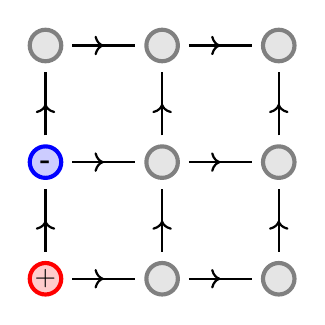
\begin{tikzpicture}[thick,decoration={
					markings,
					mark=at position 0.5 with {\arrow{>}}}
		]

		\tikzset{
			site/.style={
					circle, draw=gray, fill=gray!20, line width=1.5pt, inner sep=0pt, outer sep=4pt, minimum size=0.4cm
				},
			pcharge/.style={
					circle, draw=red, fill=red!20, line width=1.5pt, inner sep=0pt, outer sep=4pt, minimum size=0.4cm
				},
			ncharge/.style={
					circle, draw=blue, fill=blue!20, line width=1.5pt, inner sep=0pt, outer sep=4pt, minimum size=0.4cm
				},
		}
		\node[pcharge](s1){\textbf{$+$}};
		\node[site, right=0.8cm of s1](s2){};
		\node[site, right=0.8cm of s2](s3){};
		\node[ncharge, above=0.8cm of s1](s4){\textbf{-}};
		\node[site, above=0.8cm of s2](s5){};
		\node[site, above=0.8cm of s3](s6){};
		\node[site, above=0.8cm of s4](s7){};
		\node[site, above=0.8cm of s5](s8){};
		\node[site, above=0.8cm of s6](s9){};


		\draw[postaction={decorate}] (s1)--(s2);
		\draw[postaction={decorate}] (s2)--(s3);

		\draw[postaction={decorate}] (s1)--(s4);
		\draw[postaction={decorate}] (s2)--(s5);
		\draw[postaction={decorate}] (s3)--(s6);

		\draw[postaction={decorate}] (s4)--(s5);
		\draw[postaction={decorate}] (s5)--(s6);

		\draw[postaction={decorate}] (s4)--(s7);
		\draw[postaction={decorate}] (s5)--(s8);
		\draw[postaction={decorate}] (s6)--(s9);

		\draw[postaction={decorate}] (s7)--(s8);
		\draw[postaction={decorate}] (s8)--(s9);

	\end{tikzpicture}
}
\hspace{0.01\textwidth}
\subfloat[offset]{
	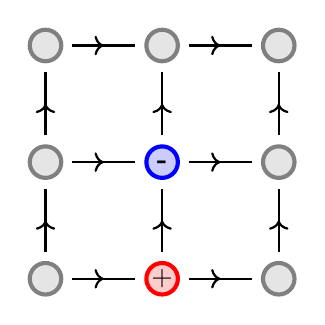
\begin{tikzpicture}[thick,decoration={
					markings,
					mark=at position 0.5 with {\arrow{>}}}
		]

		\tikzset{
			site/.style={
					circle, draw=gray, fill=gray!20, line width=1.5pt, inner sep=0pt, outer sep=4pt, minimum size=0.4cm
				},
			pcharge/.style={
					circle, draw=red, fill=red!20, line width=1.5pt, inner sep=0pt, outer sep=4pt, minimum size=0.4cm
				},
			ncharge/.style={
					circle, draw=blue, fill=blue!20, line width=1.5pt, inner sep=0pt, outer sep=4pt, minimum size=0.4cm
				},
		}
		\node[site](s1){};
		\node[pcharge, right=0.8cm of s1](s2){\textbf{$+$}};
		\node[site, right=0.8cm of s2](s3){};
		\node[site, above=0.8cm of s1](s4){};
		\node[ncharge, above=0.8cm of s2](s5){\textbf{-}};
		\node[site, above=0.8cm of s3](s6){};
		\node[site, above=0.8cm of s4](s7){};
		\node[site, above=0.8cm of s5](s8){};
		\node[site, above=0.8cm of s6](s9){};


		\draw[postaction={decorate}] (s1)--(s2);
		\draw[postaction={decorate}] (s2)--(s3);

		\draw[postaction={decorate}] (s1)--(s4);
		\draw[postaction={decorate}] (s2)--(s5);
		\draw[postaction={decorate}] (s3)--(s6);

		\draw[postaction={decorate}] (s4)--(s5);
		\draw[postaction={decorate}] (s5)--(s6);

		\draw[postaction={decorate}] (s4)--(s7);
		\draw[postaction={decorate}] (s5)--(s8);
		\draw[postaction={decorate}] (s6)--(s9);

		\draw[postaction={decorate}] (s7)--(s8);
		\draw[postaction={decorate}] (s8)--(s9);

	\end{tikzpicture}
}

		\caption{$3\cross 3$ lattice with two charge pairs of same distance but different position.}\label{fig:3x3no}
	\end{center}
\end{figure}

A clever way to avoid rims, is to use periodic boundary conditions (PBC). The disadvantage is that the shortest path is not always the path through the center links, but through the links that are introduced by the PBC. This limits our possible charge pair setups, since already for a $3 \cross 3$ lattice with PBC, there are only two different setups. All other setups can be created by translation and rotation of those two. They are depicted in \Cref{fig:3x3pbcv1}
A negative shift is expect again, since there is translational invariance. Even though it is translational invariance, it is not the same as in the continuum limit, since with PBC the paths also loop around through the links that are introduced by the PBC. Those paths are also colored in \Cref{fig:3x3pbcv1}.
The resulting potentials are marked with circles in \Cref{fig:qqbar}. The expectations are fulfilled. But the shift is even more significant then just centering the pair. The cause of this is probably the fact that with our offset setup, with a $3\cross 3$ lattice and no PBC, the one charge was still placed at a rim site. Unfortunately this cannot be avoided with a $3\cross 3$ lattice.
\begin{figure}[h]
	\begin{center}
		\subfloat[]{
			\scalebox{0.7}{
				\input{tikz/3x3pbcv1.tex}
			}
		}
		\subfloat[]{
			\scalebox{0.7}{
				\input{tikz/3x3pbcv2.tex}
			}
		}
		\caption{Two $3\cross3$ lattices with PBC and a charge pair with shortest distance (a) and second shortest distance (b). Colored paths: shortest (Green) and second shortest (Yellow) path.} \label{fig:3x3pbcv1}
	\end{center}
\end{figure}

For the continuation of the previous comparison a $4\cross4$ setup is now being used. Again, the charge pair is centered, as shown in \Cref{fig:4x4v1}. Also, only two setups are possible, where no charge is at the rim. All other can be obtained by rotating the lattice.
Since translational invariance is approached, a negative shift is expected.
\begin{figure}[h]
	\begin{center}
		\subfloat[]{
			\scalebox{0.7}{
				\input{tikz/4x4v1.tex}
			}
		}
		\subfloat[]{
			\scalebox{0.7}{
				
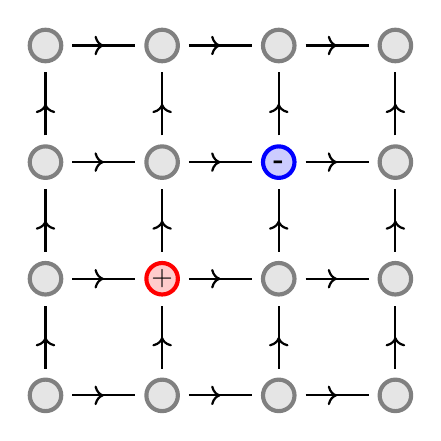
\begin{tikzpicture}[thick,decoration={
				markings,
				mark=at position 0.5 with {\arrow{>}}}
	]

	\tikzset{
		site/.style={
				circle, draw=gray, fill=gray!20, line width=1.5pt, inner sep=0pt, outer sep=4pt, minimum size=0.4cm
			},
		pcharge/.style={
				circle, draw=red, fill=red!20, line width=1.5pt, inner sep=0pt, outer sep=4pt, minimum size=0.4cm
			},
		ncharge/.style={
				circle, draw=blue, fill=blue!20, line width=1.5pt, inner sep=0pt, outer sep=4pt, minimum size=0.4cm
			},
	}
	\node[site](s1){};
	\node[site, right=0.8cm of s1](s2){};
	\node[site, right=0.8cm of s2](s3){};
	\node[site, above=0.8cm of s1](s4){};
	\node[pcharge, above=0.8cm of s2](s5){\textbf{$+$}};
	\node[site, above=0.8cm of s3](s6){};
	\node[site, above=0.8cm of s4](s7){};
	\node[site, above=0.8cm of s5](s8){};
	\node[ncharge, above=0.8cm of s6](s9){\textbf{-}};

	\node[site, above=0.8cm of s7](c1){};
	\node[site, above=0.8cm of s8](c2){};
	\node[site, above=0.8cm of s9](c3){};

	\node[site, right=0.8cm of s3](c4){};
	\node[site, right=0.8cm of s6](c5){};
	\node[site, right=0.8cm of s9](c6){};
	\node[site, right=0.8cm of c3](c7){};


	\draw[postaction={decorate}] (s1)--(s2);
	\draw[postaction={decorate}] (s2)--(s3);

	\draw[postaction={decorate}] (s1)--(s4);
	\draw[postaction={decorate}] (s2)--(s5);
	\draw[postaction={decorate}] (s3)--(s6);

	\draw[postaction={decorate}] (s4)--(s5);
	\draw[postaction={decorate}] (s5)--(s6);

	\draw[postaction={decorate}] (s4)--(s7);
	\draw[postaction={decorate}] (s5)--(s8);
	\draw[postaction={decorate}] (s6)--(s9);

	\draw[postaction={decorate}] (s7)--(s8);
	\draw[postaction={decorate}] (s8)--(s9);

	\draw[postaction={decorate}] (s7)--(c1);
	\draw[postaction={decorate}] (s8)--(c2);
	\draw[postaction={decorate}] (s9)--(c3);

	\draw[postaction={decorate}] (s3)--(c4);
	\draw[postaction={decorate}] (s6)--(c5);
	\draw[postaction={decorate}] (s9)--(c6);

	\draw[postaction={decorate}] (c3)--(c7);
	\draw[postaction={decorate}] (c6)--(c7);

	\draw[postaction={decorate}] (c1)--(c2);
	\draw[postaction={decorate}] (c2)--(c3);

	\draw[postaction={decorate}] (c4)--(c5);
	\draw[postaction={decorate}] (c5)--(c6);

\end{tikzpicture}

			}
		}
		\caption{Two $4\cross 4$ lattices with two charge pairs with shortest distance (a) and second shortest distance (b).}\label{fig:4x4v1}
	\end{center}
\end{figure}

The potential is marked with a dashed blue line in \Cref{fig:qqbar}. Comparing to the initial setup, an improvement achieved. But the difference to the $3\cross 3$ lattice with PBC is very small. It does not matter too much, that a lattice has PBC. The only importance lies in the fact, that no charges are on the rim. It would be interesting to see, if this behaviour still holds for larger lattice sizes. Unfortunately, computing those is currently not feasible.


At last a variation of the coupling is done. Already little deviations from the original coupling of $g=1$ show new behaviours. Therefore the potentials with $g=0.8$ and $g=1.2$ are compared to the original.
First $g=1.2$ is computed with the result in \Cref{fig:qqbarl}.
\begin{figure}[h]
	\begin{center}
		\includegraphics[width=0.45\textwidth]{images/quark_antiquark_potential_large_g.pdf}
	\end{center}
	\caption{Quark-Antiquark potential for different but comparable setups at $g=\num{1.2}$. By default $3\cross3$ dimensions and no PBC, if not stated otherwise.}\label{fig:qqbarl}
\end{figure}
The linearity of the potential starts to vanish and instead steps emerge, which shows that for larger couplings the lattice fragments are intensified.
A larger separation of the truncation $l=2$ and $l=3$ in respect to $l=1$ can be observed. Furthermore the potential of the $4\cross4$ lattice or the $3\cross3$ lattice with PBC is unchanged. It seems as if the truncation gains importance for larger couplings, where as the lattice size keeps its importance as is. Interestingly the potential for the centered charge pair ($l=1$, offset) moves with the $l=2$ and $l=3$ truncated potentials.

Secondly $g=0.8$ is computed with the results in \Cref{fig:qqbars}.
\begin{figure}[h]
	\begin{center}
		\includegraphics[width=0.45\textwidth]{images/quark_antiquark_potential_small_g.pdf}
	\end{center}
	\caption{Quark-Antiquark potential for different but comparable setups at $g=\num{0.8}$. By default $3\cross3$ dimensions and no PBC, if not stated otherwise.}\label{fig:qqbars}
\end{figure}
Here the $l=2$ and $l=3$ truncated potentials decrease in separation in respect to the $l=1$ truncated potential. The potential for the $4\cross 4$ and the $3\cross3$ lattice with PBC start to increase in separation in respect to the $3\cross3$ lattice with PBC and truncation $l=1$. This indicates, that as the coupling decreases the truncation looses in importance and the lattice volume, i.e. the number of total links, increases. The potential with the centered charge pair moves just as with large couplings with the truncation of $l=2$ and $l=3$. This shows that not the fact that no charge is placed on the rim is important, but the actual lattice volume.


% TODO: A $3\cross3$ lattice with $l=2$ and PBC has \num{1.9e6} physical states and takes about an hour. A $5\cross 5$ lattice with $l=1$ and no PBC has \num{}


\iffalse
	\subsection{Step scaling}
	\begin{figure}[h]
		\begin{center}
			\includegraphics[width=0.45\textwidth]{images/step_scaling.pdf}
		\end{center}
		\caption{Step scaling}
	\end{figure}
\fi

\section{Outlook}
Following the analysis of this work, the next step is to determine the running coupling, via e.g. the step scaling approach.\cite{crippa2024}

Furthermore the unit scale of the calculated quantities should be determined. Unfortunately this is not really possible for this two dimensional system, since we need to match experimental data which is measured in the real world within a 4 dimensional field theory.

To give the Hamiltonian formulation of lattice gauge theory a future, where it can be used for larger lattices, the theory needs to be implemented on a quantum computer.\cite{crippa2024} The theory can also be implemented using tensor networks.\cite{wu2025accurategaugeinvarianttensornetwork, Singh_2011}

\section{Conclusion}
With the advancemend of quantum computers, the Hamiltonian formulation of gauge theorys gains interest again. For this we started by constructing a lattice in the compact U(1) formulation where we placed electric and link operators on the links and static charges on the sites. The Kogut Susskind Hamiltonian was modefied to be in pure gauge, such that there are no fermionic fields. A truncation $l$ was introduced to render the configuration Hamiltonian finite. Further more we used Guass Law to limit our total number of configuration states to a physical subspace that later on reduces needed computational ressources.

With this theoretical setup the numerical implementation started by calculating the matrix elements for the electic and magnetic hamiltonian. Here we used the electic basis and the fact that the link operator is the canonical conjugat to the electic operator, to optain the action of our operators on our states. We briefly dived into computational ressources and build an intuition for the needed computation times.

We computed the plaquette expectation value for comparision with previous work and to confirm the correctness of the setup. Finally we computed the quark-antiquark potential by placeing two static charges. Here we measured the potential in relation to distance and experienced confinement. Further more we disscussed the influence of diffrent lattices on the potential by varying the truncation, lattice size and introducing PBC.


\begin{strip}
\section{Acknowledgements}
I want to thank Emil Rosanowski from the Funcke research group, Alessio Negro and Paul Ludwig from the Urbach research group, and of course Carsten Urbach himself, from the University of Bonn, for always being open for discussion and inspiration. I also want to thank Arianna Crippa for her code from \cite{crippa2024} to establish first intuition. 
I gratefully acknowledges the access to the Marvin cluster of the University of Bonn.
\end{strip}



\,\clearpage
\bibliography{refs}

\clearpage
\begin{textblock*}{140mm}(32.5mm, 150mm)
	Ich versichere, dass ich diese Arbeit selbstständig verfasst und keine anderen als die angegebenen Quellen und Hilfsmittel benutzt sowie die Zitate kenntlich gemacht habe.\\[40pt]
	\begin{center}
		\begin{tabular}{lr}
			Bonn, ......................................... \hspace{3cm}\, & ..................................................., \\
			\hspace{2cm}Datum                                              & Unterschrift\hspace{1.5cm}\,
		\end{tabular}
	\end{center}
	\,\\[20pt]
	1. Gutachter: Prof. Dr. Carsten Urbach \\
	2. Gutachterin: Jun.-Prof. Dr. Lena Funcke
\end{textblock*}
\end{document}
